\documentclass[11pt,a4paper]{article}

\usepackage{url}
\usepackage{graphicx}
\usepackage{amssymb}

\begin{document}

\begin{titlepage}
\thispagestyle{empty}

% Title
\vspace{10cm}
{\huge\center \bfseries  MODIM: }
\\
{\huge\center \bfseries Multi-modal Interaction Manager.}\\

{\huge\center Software description}

\vspace{5cm}
\begin{flushright}
{\large Contributors:\\
Mar\'ia T. L\'azaro\\
Federica Montesanti\\
Eugenio Sebastiani\\
Luca Iocchi}
\end{flushright}
\vfill


\end{titlepage}


%\maketitle

\newpage
\section{Introduction}
This document describes the implementation of the software component for managing multi-modal human-robot interaction. 
Concretely, a Multi-modal Interaction Manager (MODIM), a Graphical User Interface (GUI) and a speech system have been developed. These systems allow for the use of different modalities for the output and input of information from the robot to the user and viceversa. The output modalities considered are the use of texts, images or videos using the GUI or by voice using the speech synthesis. Input modalities are the touch-screen (i.e., with the use of buttons on the GUI) or spoken inputs interpreted by the speech recognizer.

\section{General Architecture}
The general architecture corresponding to the software component for multi-modal human-robot interaction is depicted in Fig. \ref{fig:architecture}. The software acts as a Multi-modal Interaction Manager (MODIM), it is implemented in Python and the source code is available in the following repository, accessible under request:
\begin{center}
  \url{https://bitbucket.org/mtlazaro/modim}
\end{center}

\begin{figure*}[!t]
\centering
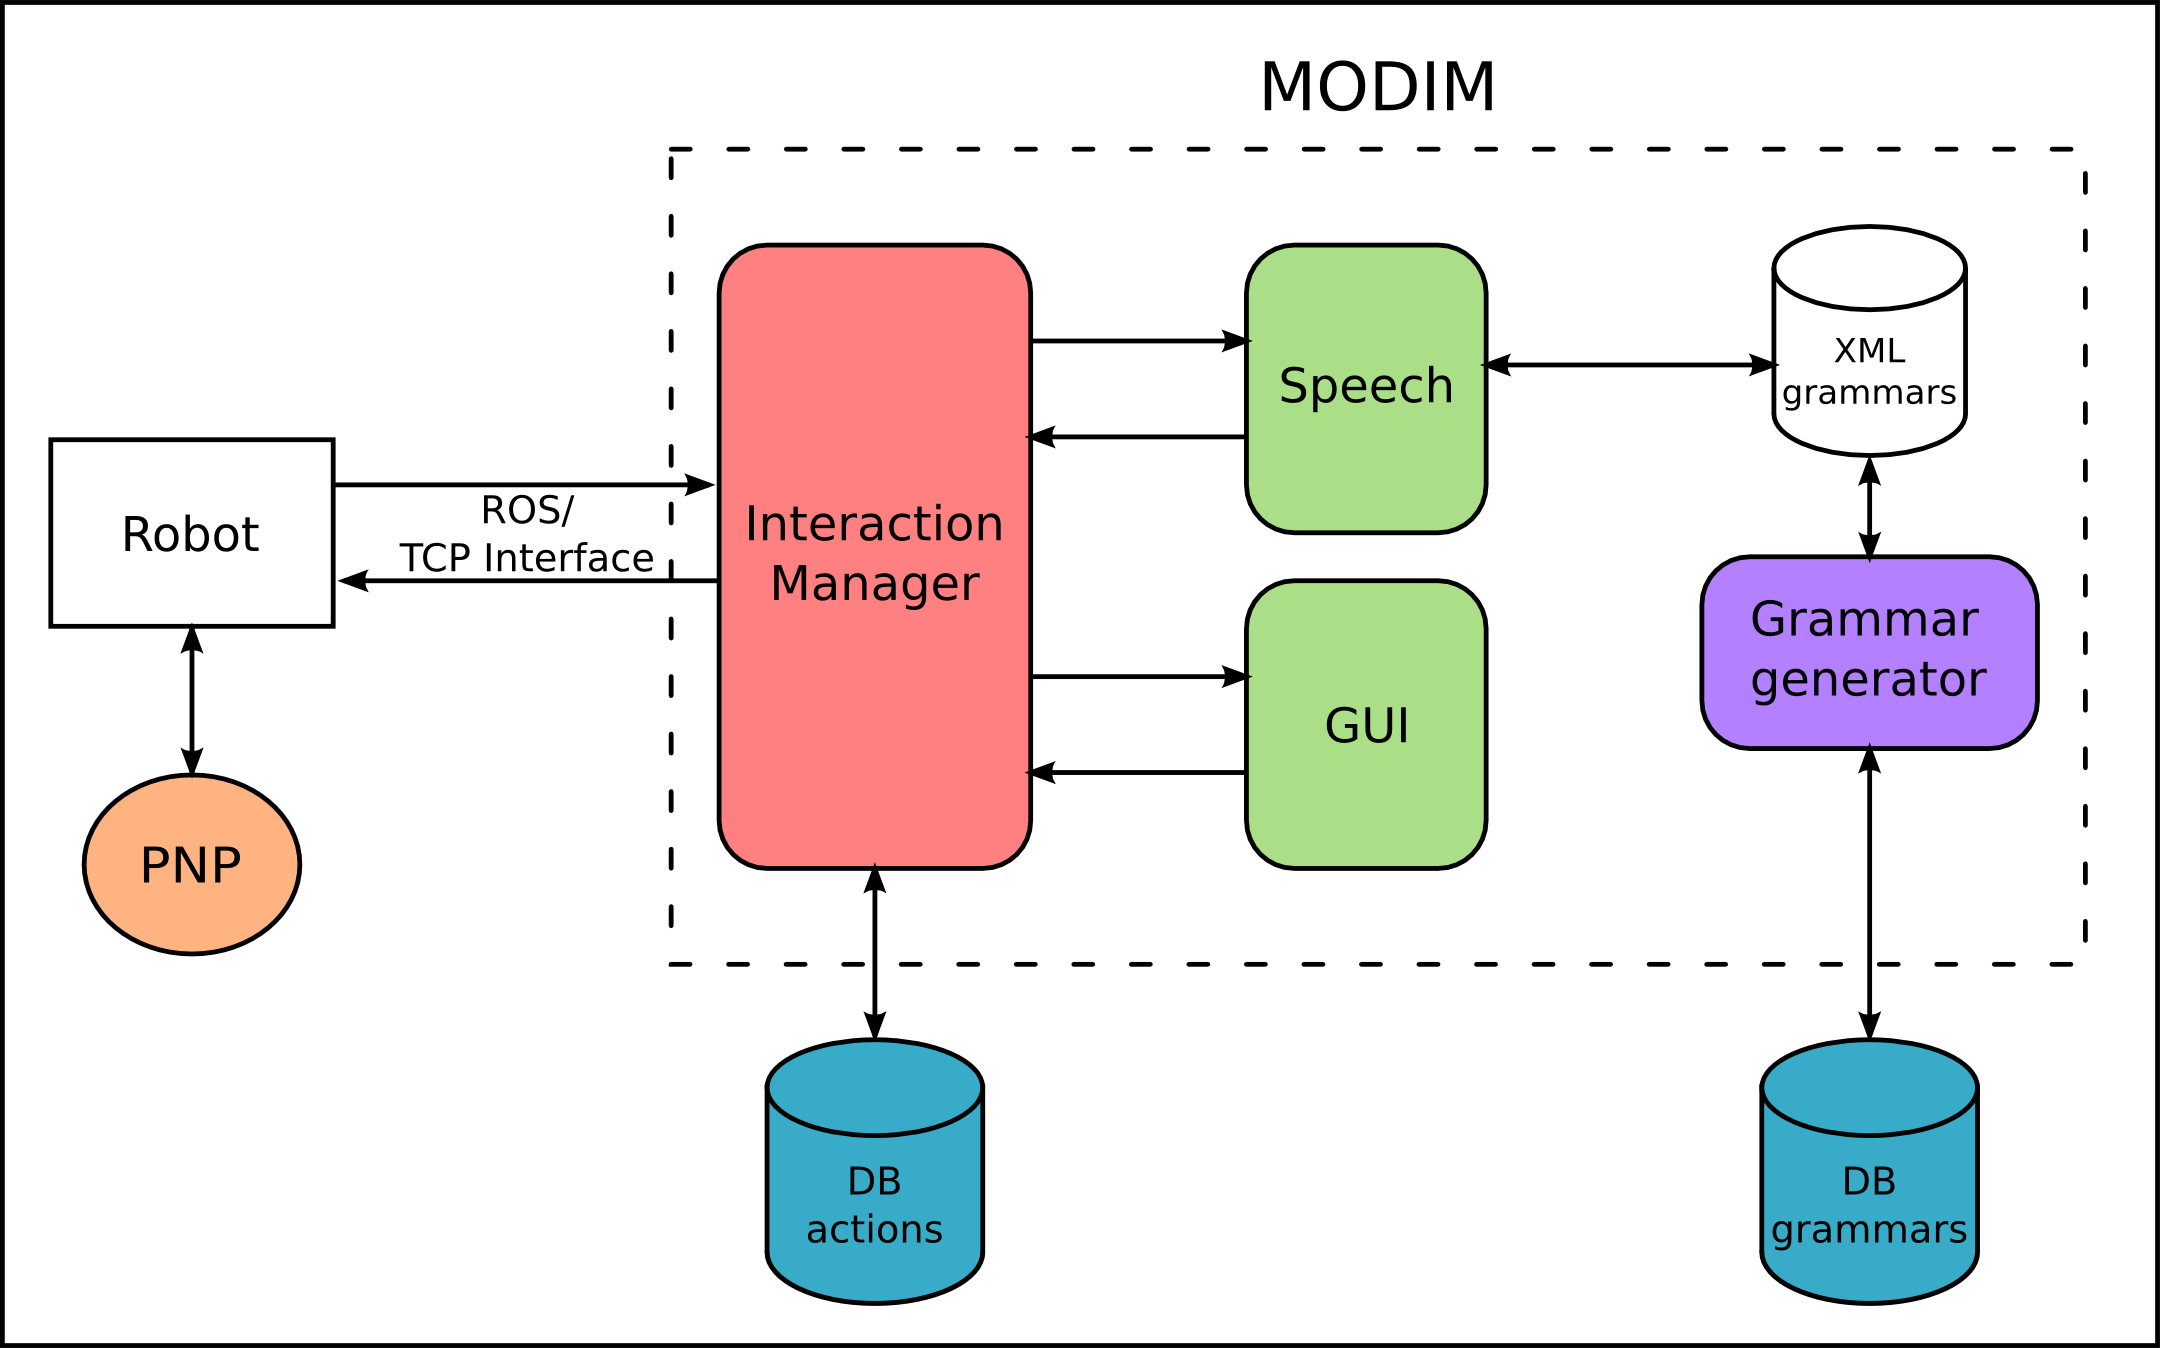
\includegraphics[width=.6\columnwidth]{img/modim.png}
\caption{Multi-modal Interaction Manager software architecture.}
\label{fig:architecture}
\end{figure*}

The MODIM software consists of three main components:
\begin{itemize}
\item \textbf{Interaction Manager.} The Interaction Manager (IM) coordinates the flow of information among the robotic modules and the human-robot interaction (GUI and speech) sub-systems. Given an interaction action coming from the PNP, the IM consults a database of actions to determine the actual content of the interaction (e.g., which concrete text or image should be displayed or spoken) and redirects the execution of the action to the GUI and/or the Speech sub-system, according to the requested modality of interaction. On the other side, the IM transmits to the robot the inputs introduced by the user through the touch-screen or via voice, which are used as conditions during the PNP execution.

\item \textbf{GUI sub-system.} The GUI sub-system is in charge of executing interaction actions that involve the display of information such as texts, images or videos. Furthermore, it captures the input from the user via the touch-screen.
Details on this sub-system are presented on Section \ref{sec:GUI}.
\item \textbf{Speech sub-system.} The Speech sub-system is in charge of executing interaction actions that involve the output of information via spoken sentences using a Text-To-Speech (TTS) component. Furthermore, the Speech sub-system is able to recognize spoken inputs from the user, whose semantic is interpreted using specific grammars contained in a database, which are enabled based on the action context. These grammars are defined in XML form, which can be written manually or automaticaly using a grammar generator that eases this process by allowing the definition of the grammars using simple text files.
Details on this sub-system are presented on Section \ref{sec:speech}
\end{itemize}

As can be observed in Fig. \ref{fig:architecture}, the MODIM software takes three different inputs: 
\begin{itemize}
\item A \textbf{PNP} to describe the robot behaviour. Confer the PNP documentation\footnote{http://pnp.dis.uniroma1.it} for the definition of the PNP.
\item The definition of the \textbf{actions}. This will be explained in Section \ref{sec:actiondef}.
\item The definition of the \textbf{grammars}. This will be explained in Section \ref{sec:grammardef}.
\end{itemize}

\section{Interaction Manager}
\label{sec:IM}
The Interaction Manager (IM) coordinates the flow of information among the robotic modules and the human-robot interaction (GUI and speech) sub-systems. On one side, the IM receives the actions corresponding to interaction routines contained in the input PNP, which is executed on the robot. Given an interaction action, the IM consults a database of actions to determine the actual content of the interaction (e.g., which concrete text or image should be displayed or spoken) and redirects the execution of the action to the GUI and/or the Speech sub-system, according to the requested modality of interaction. On the other side, the IM receives from the GUI and Speech sub-systems inputs introduced by the user (e.g., through the touch-screen or via voice), which are transmitted to the robot and used as conditions during the PNP execution. The IM allows for a transparent management of the input modalities from the user point of view, i.e., when a condition in the PNP must be enabled by the answer of the user, it can arrive indistinctly from the speech or the touch-screen.

This coordination is reached by using 2 separate threads which implement: 1) a TCP client for the ROS server running on the robot, which sends to the IM the actions contained in the PNP corresponding to interaction routines and 2) a TCP client connecting to the speech server to receive the recognized words by the Automatic Speech Recognition component and to send requests for executing TTS actions and loading specific grammars according to the action in course. Communicaton with the GUI sub-system is done by means of events sent between the Python classes that implement the ROS TCP client and the GUI. These events control the time in which each area of the GUI layout must be updated with the information of the action.

Currently, the IM accepts the interaction instructions from the PNP execution manager summarized in Table \ref{tab:PNPInstructionsSupported}.
 \begin{table}[h]
\begin{center}
  \begin{tabular}{| l | c | c |}
    \hline
    \textbf{PNP Action} & \textbf{GUI} &  \textbf{Speech}\\ \hline
    $display\_text\_interactionname$ & \checkmark & Optional\\ \hline
    $display\_image\_interactionname$ & \checkmark & \\ \hline
    $display\_txtimg\_interactionname$ & \checkmark & Optional\\ \hline
    $ask\_interactionname$ & \checkmark & Optional\\ \hline
    $askimg\_interactionname$ & \checkmark & Optional\\ \hline
    $say\_interactionname$ & & \checkmark\\ \hline
    $display\_init$ & \checkmark & Optional\\
    \hline
  \end{tabular}
\end{center}
    \caption{PNP actions currently supported by the system and sub-systems involved for each one.}
    \label{tab:PNPInstructionsSupported}   
\end{table}

Interaction actions are grouped in three main types: $display, ask$ and $say$ whose execution on the GUI or/and on the Speech sub-system varies on the action as shown in Table \ref{tab:PNPInstructionsSupported}.  
The most basic function is defined as:
$$display\_mode\_interactionaction$$
where $mode$ can be set to $[text|image|txtimg]$ to update the corresponding reserved area of the GUI interface for that modality of interaction, displaying the content of an action description file with name $mode\_interactionaction$. We consider it is a pleasant behaviour from the robot to speak texts displayed on the GUI. For that reason, $display$ actions with $text|txtimg$ modality also involve by default the use of the Speech sub-system. However, this behaviour is optional depending on the definition of the action. More details on this definition will be given on Section \ref{sec:actiondef}.

Many types of interactions involve to formulate a question to the user (e.g., to find out her/his needs) and present to her/him some possible choices. We contemplate this type of interaction with the definition of a higher level function:
$$[ask|askimg]\_interactionaction$$
for which the display of a text (i.e., the question) in the case of the $ask$ function or a text plus an image ($askimg$) is done, together with the display of a set of buttons containing the set of possible answers from the user. Again, the TTS is also activated by default during the display of the text, although can be optionally deactivated. Buttons will be displayed only when the Speech sub-system has finished the synthesis of the spoken question. This event is notified by the Speech sub-system by sending the command [END\_SYNTH] to the interaction manager.  

Furthermore, action $say\_interactionname$ has been inherently defined to speak a text without visualizing it, therefore, only the Speech sub-system is involved in this case.

Finally, a function $display\_init$ is used to restart the GUI and the Speech sub-systems to their idle state, i.e., when the robot is not interacting with a user. This involve to show a specific content on the GUI or to load an initial grammar on the Speech sub-system.
This information is established through a configuration file $init$ whose content and definition will be explained in Section \ref{sec:actiondef}.

\section{GUI sub-system}
\label{sec:GUI}
The GUI sub-system implements a graphical input and output interface between users and robots. 
It is implemented in Python using the TkInter package, a cross-platform GUI builder.

Figure \ref{fig:GUIlayout} shows the basic layout of the graphical user interface. As can be seen in the figure, each form of interaction has a reserved space on the displayed window. Output interactions from the robot to the user using the GUI are in form of texts, images and videos while a reseved space for buttons is used to accept input interactions from the user. Additionally, a language selection button is available for multi-language interaction, allowing for a more personalized human-robot interaction. Figure \ref{fig:GUIInstances} shows examples of the Graphical User Interface.

Coordination between the GUI sub-system and the IM is done by means of events generated by the IM. Each one of these events is associated to the widget that controls each reserved space of the GUI (i.e., the text, image and buttons area). Table \ref{tab:PNPGUIeventsrelation} summarizes which events are generated upon reception of each PNP GUI actions.

\begin{table}[h]
\begin{center}
  \begin{tabular}{| l | l |}
    \hline
    \textbf{PNP GUI Action} & \textbf{Event Generated from IM to GUI} \\ \hline
    $display\_text\_interactionname$ & {\ttfamily <<NewTextMessage>>} \\ \hline
    $display\_image\_interactionname$ & {\ttfamily <<NewImgMessage>>} \\ \hline
    $display\_txtimg\_interactionname$ & {\ttfamily <<NewTextMessage>>} \\
    & {\ttfamily <<NewImgMessage>>}\\ \hline
    $ask\_interactionname$ & {\ttfamily <<NewTextMessage>>}\\
    & {\ttfamily <<NewButtonsMessage>>}\\ \hline
    $askimg\_interactionname$ & {\ttfamily <<NewTextMessage>>} \\
    & {\ttfamily <<NewImgMessage>>}\\
    & {\ttfamily <<NewButtonsMessage>>}\\ \hline
    $display\_init$ & {\ttfamily <<resetMessage>>} \\
    \hline
  \end{tabular}
\end{center}
    \caption{Events generated from the IM to update the GUI for each PNP GUI instruction.}
    \label{tab:PNPGUIeventsrelation}   
\end{table}

\begin{figure*}[!t]
\centering
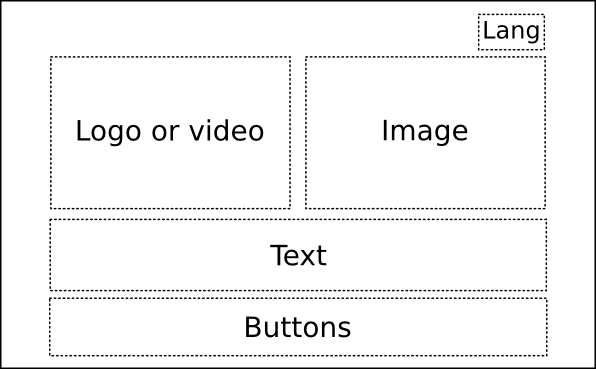
\includegraphics[width=.6\columnwidth]{img/GUIlayout.png}
\caption{Layout of the Graphical User Interface.}
\label{fig:GUIlayout}
\end{figure*}

\begin{figure*}[!t]
\centering
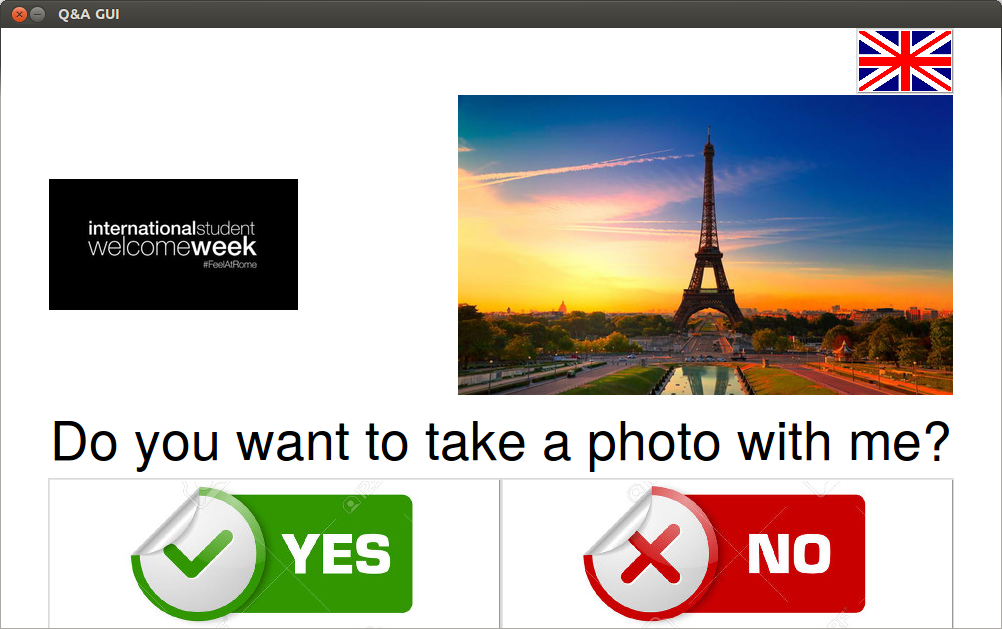
\includegraphics[width=.45\columnwidth]{img/erasmus_wantphoto.png}
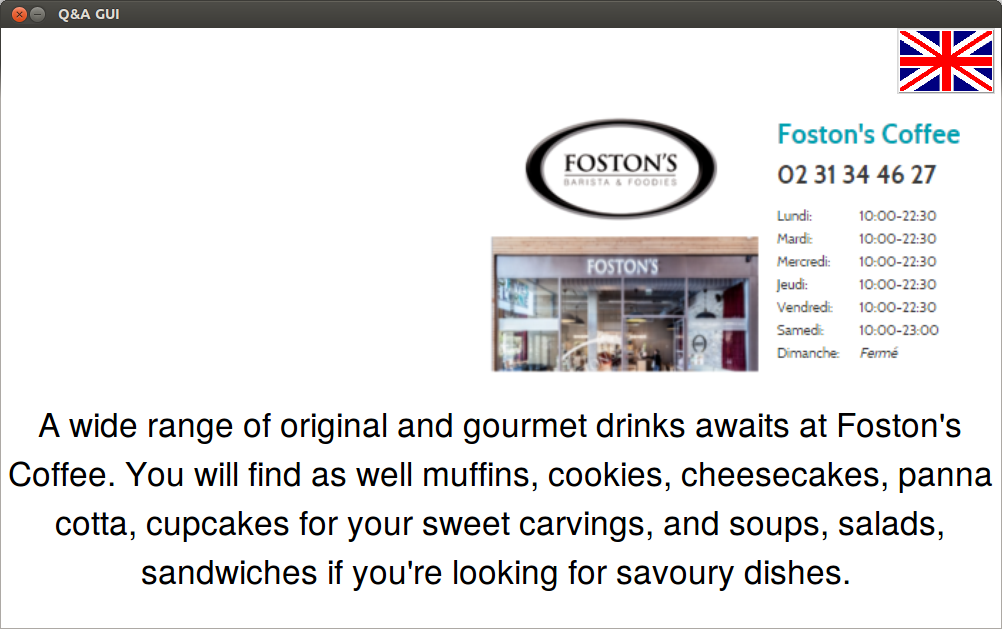
\includegraphics[width=.45\columnwidth]{img/fostons.png}
\caption{Instances of the Graphical User Interface.}
\label{fig:GUIInstances}
\end{figure*}

\section{Speech sub-system}
\label{sec:speech}
The speech sub-system allows the robot to communicate with humans through vocal interactions. It is
formed by two main components: Automatic Speech Recognition (ASR) and Text-To-Speech (TTS).
The ASR component analyzes audio data coming from a microphone and extract semantic information about the spoken sentences, according to a predefined grammar. This component allows the robot to understand user spoken commands. The speech recognition module is based on the Microsoft Speech platform and on a further processing module that builds the semantic frames of the recognized sentences.

The TTS component transforms text messages in audio data that are then emitted by the speakers
on-board the robot. This enables the robot to speak to people. The Microsoft TTS engine is used for
this module.

The speech software is multilingual. Currently, it supports English, French, Italian and Spanish but it can be easily extended to manage other languages, upon installation of the corresponding language package of the Microsoft engine in the system.

The software is implemented as a TCP server that accepts commands to load specific grammars for the ASR component or to speak a text with the TTS component.
Concretely, these commands and their syntax is the following:
\begin{itemize}
\item {[LOAD\_GRAMMAR]} $<grammar\_name> |$ locale
\item {[SAY]} $<\emph{text-to-speech}> |$ locale
\end{itemize}
where locale (e.g., en, fr, it, es) is a string to specify the language of the speech recognition or the TTS engine.

\section{Action definition}
\label{sec:actiondef}

Currently, the IM can interpret the following set of instructions coming from the PNP:
\begin{itemize}
\item $display\_mode\_interactionname$, where $mode=[text|image|txtimg]$
\item $[ask|askimg]\_interactionname$
\item $say\_interactionname$
\item $display\_init$
\end{itemize}

Once the IM receives one of these instructions, it needs to 'ground' the actions to the current context. To this end, the IM consults a DB of actions where actions are described in the form of text files. 
The syntax used in these text files is simple and easy to read and write by non-expert users.
The text files must be named with the format \textbf{[text$|$image]\_interactionname} and their relation with the PNP instructions is summarized in Table \ref{tab:PNPtextfilerelation}. Action $display\_init$ is a special function which requires a configuration file called \textbf{init} which requires a different syntax also explained next in this section.
\begin{table}[h]
\begin{center}
  \begin{tabular}{| l | l |}
    \hline
    \textbf{PNP Action} & \textbf{Action file required} \\ \hline
    $display\_text\_interactionname$ & text\_interactionname \\ \hline
    $display\_image\_interactionname$ & image\_interactionname \\ \hline
    $display\_txtimg\_interactionname$ & text\_interactionname \\
    & image\_interactionname\\ \hline
    $ask\_interactionname$ & text\_interactionname \\ \hline
    $askimg\_interactionname$ & text\_interactionname \\
    & image\_interactionname\\ \hline
    $say\_interactionname$ & text\_interactionname \\\hline
    $display\_init$ & init \\
    \hline
  \end{tabular}
\end{center}
    \caption{Required action text files for each PNP instruction.}
    \label{tab:PNPtextfilerelation}   
\end{table}

Next, we provide the syntax for each of these text files.
\begin{itemize}
\item \textbf{text\_interactionname}: action files with text modality are organized in three different sections:
{\ttfamily
\begin{center}
  \begin{tabular}{|l|}
    \hline
rules text section\\
----\\
BUTTONS\\
rules buttons section\\
----\\
ASRCMD\\
rules grammar section\\
    \hline
  \end{tabular}
\end{center}
}
where buttons and grammar sections are only required when the interaction action expects an answer from the user (i.e., $ask$ and $askimg$ PNP actions) that can be either through the touch screen or spoken. In that case, the IM coordinates the display of a set of buttons on the GUI and enables a specific grammar in the speech system for speech recognition.

\item \textbf{image\_interactionname}: action files with image modality only contain one section corresponding to the rules to select the image to be displayed.
{\ttfamily
\begin{center}
  \begin{tabular}{|l|}
    \hline
rules image section\\
    \hline
  \end{tabular}
\end{center}
}
\end{itemize}

Each section contains a list of rules which allow for personalization and variability according to a given profile.
A single rule has the format:
\[\tt profile : actual\_action \]
where {\tt profile} is a tuple of the form {\tt<age,gender,language,occupation>} and {\tt actual\_action} can be either a text or a path to an image to be displayed or a command for the speech system. For some actions, not all the profile fields are required to be known. In that case we use the symbol '*' to denote an unknown or not required field.
For example, the image shown by the robot to give information about the toilets location in an office environment could only depend on the gender of the user. For the case of a female user, the following rule could be arranged:
\[\tt<*,female,*,*>: path\_to\_women\_toilets\_image\]

Furthermore, as mention before, the texts that are displayed are also spoken by default. However, we can specify different texts to be displayed or spoken. To this end, we use the following syntax:
\[\tt profile : text\_to\_display | text\_to\_TTS \]
where {\tt text\_to\_TTS} can also be empty and, in that case, the text will be displayed but not spoken.

Each text, image and grammar section contains a list of these rules. Buttons section is more complex since we define a list of rules for each button as shown below. The content to be displayed in the buttons can be either text or an image.
{\ttfamily
\begin{center}
  \begin{tabular}{|l|}
    \hline
button\_1\\
rules button\_1\\
button\_2\\
rules button\_2\\
\vdots\\
    \hline
  \end{tabular}
\end{center}
}

Table \ref{tab:textFileExample} shows an example of a text file to describe the action {\tt ask\_whichcolor}, in which the user is inquired about its favourite color. In this example, different rules are described depending on the language. Finally, Table \ref{tab:imageFileExample} shows an example of a text file to describe the action {\tt display\_image\_toilet}, in which personalization is done base on the gender.
\begin{table}[h]
{\ttfamily
\begin{center}
  \begin{tabular}{|ll|}
    \hline
<*,*,es,*>: &"¿Cuál es tu color preferido?"\\
<*,*,*,*>:  &"What is your favourite color?"\\
----&\\
BUTTONS&\\
green&\\
<*,*,es,*>: &Verde\\
<*,*,*,*>:  &Green\\
blue&\\
<*,*,es,*>: &Azul\\
<*,*,*,*>:  &Blue\\
red&\\
<*,*,es,*>: &Rojo\\
<*,*,*,*>:  &Red\\
yellow&\\
<*,*,es,*>: &Amarillo\\
<*,*,*,*>:  &Yellow\\
orange&\\
<*,*,es,*>: &Naranja\\
<*,*,*,*>:  &Orange\\
white&\\
<*,*,es,*>: &Blanco\\
<*,*,*,*>:  &White\\
black&\\
<*,*,es,*>: &Negro\\
<*,*,*,*>:  &Black\\
----&\\
ASRCMD&\\ 
<*,*,es,*>: &[LOAD\_GRAMMAR] frame\_colornames|es\\
<*,*,*,*>:  &[LOAD\_GRAMMAR] frame\_colornames\\
    \hline
  \end{tabular}
\end{center}
}
    \caption{Example of text file to define an $ask$ action.}
    \label{tab:textFileExample}   
\end{table}

\begin{table}[h]
{\ttfamily
\begin{center}
  \begin{tabular}{|ll|}
    \hline
<*, m, *, *>:  &"img/men\_toilets.png"\\
<*, f, *, *>:  &"img/women\_toilets.png"\\
<*, *, *, *>:  &"img/default\_toilets.png"\\
    \hline
  \end{tabular}
\end{center}
}
    \caption{Example of text file to define a $display\_image$ action.}
    \label{tab:imageFileExample}   
\end{table}

As mentioned before, action {\tt display\_init} is used to restart the state of the GUI and Speech sub-systems. It requires the defition of an \textbf{init} configuration file containing the following information:
\begin{itemize}
\item WELCOMEMSG: Text message to be displayed on the idle state of the robot, i.e., when no interaction is being realized.
\item LEFTIMG: Image/video to be displayed on the left side of the GUI. It remains fixed during the interaction.
\item RIGHTIMG: Image to be displayed on the right side of the GUI. It is changed during the interaction.
\item PROFILE: Default profile with format <age, gender, language, occupation>
\item MULTILANG: set to YES if multiple languages must be considered. In that case the Lang button is displayed on the GUI.
\item GRAMMAR: Grammar that must be loaded at the beginning of the interaction.
\end{itemize}


\section{Grammar definition}
\label{sec:grammardef}

A grammar contains a set of rules that specify the spoken words and phrases that the speech recognition engine can recognize. The syntax used for representing grammars follows the Speech Recognition
Grammar Specification (SRGS) developed by the World Wide Web Consortium (W3C) which uses the XML language.

However, writting a grammar is time consuming and error-prone since the syntax and the structure of a grammar document requires a good knowledge about the SRGS and XML.

For these reasons we developed a module referred as Grammar Generator (see Fig. \ref{fig:architecture}) able to generate XML grammar files from simple text files.

The text file encloses all the words, sequence of words or phrases to be recognized
by the ASR given a certain topic. Its name is exactly the name of the topic of interest: \textbf{topic.txt}.
This text file is the only file to be written or to be modified in order to create, to
add or to delete elements from a grammar.

Each line of these text files defines a rule of the grammar. More specificaly, each line contains a structure ``{\ttfamily words/phrases to be recognized -> semantic symbol}''.
Table \ref{tab:grammarFileExample} (left) shows an example of the content of a text file to generate a grammar.

It is necessary to create different grammars for each language that we want to consider, since a unique locale must be established on the SRGS format. 
We consider the multi-language case by specifying the locale as a part of the name of the .txt file (\textbf{topic\_locale.txt}). If no locale is specified in the name of the file (as in the case of Table \ref{tab:grammarFileExample}, right), the designated locale is the English one (en-US).  
Table \ref{tab:grammarFileExample} (left) shows the equivalent text file to create a grammar on the topic confirm in Spanish. Notice how the semantic symbols remain the same independently of the language.

\begin{table}[h]
{\ttfamily
\begin{center}
  \begin{tabular}{|l|}
    \hline
\bf{confirm.txt} \\
    \hline
yes -> yes\\
no  -> no \\
cancel, sorry I made a mistake -> cancel \\
    \hline
\bf{confirm\_es-ES.txt}\\
    \hline
si -> yes\\
no -> no\\
cancelar, lo siento me he equivocado -> cancel \\
    \hline
  \end{tabular}
\end{center}
}
    \caption{Examples of text file to generate a grammar on the topic confirm. Top: english grammar. Bottom: spanish equivalent grammar.}
    \label{tab:grammarFileExample}   
\end{table}



\end{document}
